%!TEX root = ../../thesis.tex
\chapter{Quantifying Reticulation Using Topological Complex Constructions}
\label{ch:complex_construction}

In Chapter \ref{ch:background}, phylogenetic networks were introduced as a generalization of phylogenetic trees as a way of representing reticulation in an evolutionary dataset.
In this Chapter, we introduce a construction for phylogenetic networks and show how it 

\section{Introduction}
\label{sec:introduction}

The application of persistent homology to molecular sequence data was introduced in \autocite{Chan:2013}, where recombination rates in viral populations were estimated by computing $L_p$ norms on barcode diagrams.
In that paper, it was shown that persistent homology provides an intuitive quantification of reticulate evolution in sequence data by measuring deviations from tree-like additivity.
Reticulation is manifest as nonvanishing higher homology ($H_{n}>0$ for $n>0$) in the filtration.
Using persistent homology asa tool to measure reticulate evolution is useful because it

\begin{inparaenum}[(1)]
\item provides a method of quantifying the extent of reticulation, and
\item provides a method of tracking the scale of reticulate events.
\end{inparaenum}

Our goal is to more clearly understand the topological signal that persistent homology captures when applied to sequence data.
In doing so, we construct simple examples in which a genetic distance filtration is insensitive to reticulation.

Due to the coarseness of the distance filtration, only those reticulations which have sufficiently strong support in the sequence data will be detected.
By coarseness, we mean that thae distance filtration...
Small distortions in the metric space, due possibly to incomplete population sampling or weakly supported reticulations, will reduce sensitivity.
Looking to increase the resolution of our approach led us to consider a class models which construct a \emph{median graph} from a set of sequences.
Median graphs form the basis for a large number of phylogenetic network algorithms and have been extensively studied over the past several decades \autocite{Bandelt:1999}.
The approach is closely related to split decomposition, and it can be shown that the objects resulting from the two methods are identical \autocite{Bandelt:1992}.
The median graph approach imputes putative evolutionry ancestors into the set of vertices, and forms a network representing the incompatibile splits present in the sequence data.
A common task has been to quantify the complexity of the resulting network.
We show that a filtration of complexes built from the median graph vertex set is a fast an efficient way to characterize the complexity of a phylogenetic network.
Due to a result of Gromov, we know that the complexes built on this vertex set will be cubical, making the barcode diagram simple to interpret \citet{Gromov:1987}.

Additionally, we sought to more clearly interpret nontrivial higher homology ($H_{n}$ for $n>1$) in the barcode diagram.
In \citet{Chan:2013}, higher homology was presented as evidence for complex reticulations.
An application to the 2013 H7N9 influenza epidemic was presented, where the source of the epidemic was shown to be the result of a triple reassortment from three parental strains.
The triple reassortment was 
We expand on this idea, identifying conditions for which higher homology will be observed.
These conditions take the form of analogues of the classical four-gamete test.
Relationships between the homology dimension and the number of haplotypes are suggested.
To simplify the intepretation of higher homology, we introduce a new construction for building \Cech\ complexes on binary sequence data.

In this paper we present three ideas to increase the usefulness of the signal generated by persistent homology.

The structure of this paper is as follows.
In Section \ref{sec:background} we review the application of persistent homology to sequence data.
We present simple examples in which the genetic distance filtration fails to capture reticulation.
In Section \ref{sec:median_complex} we present the median closure of the original vertex set.
We show how this operation recovers invariant signals of incompatibility in a quantitative way.
In Section \ref{sec:higher_homology} we discuss interpretations of higher dimensional homology and introduce a \Cech\ complex construction on sequence data.
% In Section \ref{sec:cech_complex} we present
In Section \ref{sec:examples} we present examples of our approach.
Throughout, we assume biallelic data under an infinite sites model with no back mutation.

\section{Persistent Homology of Sequence Data}
\label{sec:background}

In this section we briefly review the ideas in \citet{Chan:2013} as they relate to the application of persistent homology to sequence data.

\subsection{Vertical Evolution}
\label{subsec:vertical_evolution}
%
In the standard model of evolution, novel genotypes arise via mutation during reproduction.
In this case, evolutionary relationships will be accurately modeled as a bifurcating tree.
The distance matrix generated from such sequence data will have the property that it is additive.
An additive metric can be written as a bifurcating tree such that the distance between any two points in the metric is equal to the path distance along the tree.

To check that a given metric is additive, it is sufficient to check the \emph{four point condition}.
The four point condition says that for every set of four points in the data, there is an ordering on the points such that
\begin{equation}
d_{ij}+d_{kl} \leq d_{ik}+d_{jl} = d_{il}+d_{jk}.
\end{equation}

Consider the example in Figure \ref{fig:fig1_sequences}.
This set of five sequences can be represented the tree in Figure \ref{fig:fig1_tree}.
The barcode diagram from a persistent homology computation is shown in Figure \ref{fig:fig1_barcode}.

% \begin{figure}
%   \centering
%   \fbox{\begin{subfigure}[c]{0.3\textwidth}
%     \begin{align*}
%       s_{1} & = 1100000 \\
%       s_{2} & = 1010000 \\
%       s_{3} & = 0001000 \\
%       s_{4} & = 0000110 \\
%       s_{5} & = 0000101
%     \end{align*}
%     \caption{Sequences}
%     \label{fig:fig1_sequences}
%   \end{subfigure}}
%   ~
%   \fbox{\begin{subfigure}[c]{0.3\textwidth}
%     \begin{tikzpicture}
%       \coordinate (0) at (0,0);
%       \coordinate[label=270:$s_3$] (1) at (0,-1);
%       \coordinate (2) at (-1,0);
%       \coordinate (3) at (1,0);
%       \coordinate[label=45:$s_4$] (4) at (1.707,0.707);
%       \coordinate[label=-45:$s_5$] (5) at (1.707,-0.707);
%       \coordinate[label=135:$s_1$] (6) at (-1.707,0.707);
%       \coordinate[label=-135:$s_2$] (7) at (-1.707,-0.707);
%       \draw[black,thick] (6) -- (2) -- (0) -- (3) -- (4);
%       \draw[black,thick] (7) -- (2) -- (0) -- (3) -- (5);
%       \draw[black,thick] (0) -- (1);
%     \end{tikzpicture}
%     \caption{Tree}
%     \label{fig:fig1_tree}
%   \end{subfigure}}
%   ~
%   \fbox{\begin{subfigure}[c]{0.3\textwidth}
%     %\includegraphics[width=\textwidth]{fig/fig1_barcode.eps}
%     \caption{Barcode}
%     \label{fig:fig1_barcode}
%   \end{subfigure}}
%   \caption{A tree is trivially contractible and has vanishing higher homology.}
%   \label{fig:fig1}
% \end{figure}

\begin{figure}
  \centering
  \fbox{
  \subbottom[Sequence]{
    \begin{tabular}{lc}
    $s_{1}$ & = 1100000 \\
    $s_{2}$ & = 1010000 \\
    $s_{3}$ & = 0001000 \\
    $s_{4}$ & = 0000110 \\
    $s_{5}$ & = 0000101
    \end{tabular}
      % \begin{align*}
      % s_{1} & = 1100000 \\
      % s_{2} & = 1010000 \\
      % s_{3} & = 0001000 \\
      % s_{4} & = 0000110 \\
      % s_{5} & = 0000101
      % \end{align*}
    \label{fig:fig1_sequences}
  }}
  ~%\hfill
  \fbox{
  \subbottom[Tree]{
      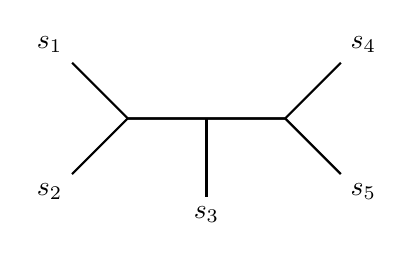
\begin{tikzpicture}
      \coordinate (0) at (0,0);
      \coordinate[label=270:$s_3$] (1) at (0,-1);
      \coordinate (2) at (-1,0);
      \coordinate (3) at (1,0);
      \coordinate[label=45:$s_4$] (4) at (1.707,0.707);
      \coordinate[label=-45:$s_5$] (5) at (1.707,-0.707);
      \coordinate[label=135:$s_1$] (6) at (-1.707,0.707);
      \coordinate[label=-135:$s_2$] (7) at (-1.707,-0.707);
      \draw[black,thick] (6) -- (2) -- (0) -- (3) -- (4);
      \draw[black,thick] (7) -- (2) -- (0) -- (3) -- (5);
      \draw[black,thick] (0) -- (1);
      \end{tikzpicture}
      \label{fig:fig1_tree}
  }}
  ~%\hfill
  \fbox{
  \subbottom[Barcode]{
    %\includegraphics[width=\textwidth]{fig/fig1_barcode.eps}
    \label{fig:fig1_barcode}
  }}
  \caption{A tree is trivially contractible and has vanishing higher homology.}
  \label{fig:fig1}
\end{figure}

A tree is trivially contractible, and hence has vanishing higher homology.
This result was proven for sequence data in \citep{Chan:2013}.
In practice, most data is not additive.
The field of phylogenetics is essentially tasked with finding the \emph{best} tree given sequence data, for some notion of best.

\subsection{Reticulate Evolution}
\label{subsec:reticulate_evolution}
%
Reticulate, or horizontal, evolution refers to any evolutionary process by which genetic material is transfered between organisms in a method other than asexual reproduction.
Examples include species hybridization, bacterial gene transfer, and homologous recombination.
In these situations, no tree can be drawn that accurately reflects the evolutionary history of a set of sequences.

A simple test for the presence of reticulation is given by the \emph{four gamete test}.
The four gamete test states that the simultaneous presence of haplotype patterns 00, 01, 10, and 11 is incompatible with strictly vertical evolution in an infinite sites model.
It provides direct evidence for reticulate evolution.
One way to quantify recombination in a set of sequences is the Hudson-Kaplan test, which counts the minimum number partitions required in the data such that within each partition the all sites are compatible \citep{Hudson:1985}.

We consider the four gametes to be the fundamental unit of recombination.
Topologically, this unit represents a loop.
In a persistent homology computation, we would see nonvanishing $H_1$ homology in the interval $[1,2)$ (see Figure XXX).

% \begin{figure}
%   \centering
%   \fbox{\begin{subfigure}[c]{0.3\textwidth}
%     \centering
%     \begin{align*}
%       s_{1} & = 00 \\
%       s_{2} & = 10 \\
%       s_{3} & = 01 \\
%       s_{4} & = 11
%     \end{align*}
%     \caption{Sequences}
%     \label{fig:fig2_sequences}
%   \end{subfigure}}
%   ~
%   \fbox{\begin{subfigure}[c]{0.3\textwidth}
%   \centering
%   \begin{tikzpicture}
%     \centering
%     \coordinate[label=90:00] (0) at (0,0);
%     \coordinate[label=0:01] (1) at (1,-1);
%     \coordinate[label=180:10] (2) at (-1,-1);
%     \coordinate[label=-90:11] (3) at (0,-2);

%     \draw[black, thick] (0) -- (1) -- (3) -- (2) -- cycle;
%     \foreach \i in {0, 1, 2, 3} {
%       \draw[fill=black] (\i) circle (0.15em);
%     }
%   \end{tikzpicture}
%   \caption{Loop}
%   \label{fig:fig2_loop}
%   \end{subfigure}}
%   ~
%   \fbox{\begin{subfigure}[c]{0.3\textwidth}
%     %\includegraphics[width=\textwidth]{fig/fig2_barcode.eps}
%     \caption{Barcode}
%     \label{fig:fig2_barcode}
%   \end{subfigure}}
%   \caption{The fundamental unit of reticulation is the loop given by the four gamete test.}
%   \label{fig:fig2}
% \end{figure}

In the fundamental loop, we can give an interpretation to each vertex.
There is a common ancestor, two parents, and a recombinant child.
Of course, we do not \emph{a priori} know which sequences played which role in a given loop, which is the same as the problem of rooting a phylogenetic tree.
Persistent homology is simply a method of efficiently counting the number of such loops in the data, across all genetic scales.

\section{Examples}
\label{sec:examples}

In considering small examples of this form we often encountered cases in which the four gamete test indicated reticulation, but persistent homology failed to detect a loop.
What these examples had in common is that due to distortion in the metric space, simplices would collapse before they should have.
This could have been due to incomplete population
This could have been due to incomplete sampling, in which case recombination fails to be detected because parental sequences collapse to early, or due to cases where recombination creates new sequences that sit intermediate to parental and ancestral sequences.
Here we work through two examples in detail.

\paragraph{Example 1}
\label{ex:example1}
%
It is generally the case that we do not have a complete sampling of the sequences corresponding to the evolutionary history of a set of sequences.
For example, we may not have sampled the true recombinant child, only a descendant which has accumulated additional mutations.
Consider the set of sequences 000, 100, 010, and 111.
From the four-gamete test we know there is an incompatibility between sites 1 and 2, indicating the presence of a reticulate event.
Let us arbitrarily choose $s_1$ to be the common ancestor, $s_2$ and $s_3$ to be parents, and $s_4$ to be a descendant of the reticulate event.
We can infer that the recombinant was of the form $s_r=110$.
Unfortunately, the persistent homology the four sequences will be trivial.
To understand why, consider an embedding of the four sampled sequences onto the 3-cube, as seen in Figure XXX.

% \begin{figure}
%   \centering
%   \fbox{\begin{subfigure}[c]{0.3\textwidth}
%     \centering
%     \begin{align*}
%       s_{1} & = 000 \\
%       s_{2} & = 100 \\
%       s_{3} & = 010 \\
%       s_{4} & = 111
%     \end{align*}
%     \caption{Sequences}
%     \label{fig:fig3_sequences}
%   \end{subfigure}}
%   ~
%   \fbox{\begin{subfigure}[c]{0.3\textwidth}
%     \centering
%     \definecolor{light-gray}{gray}{0.85}
%     \begin{tikzpicture}
%       \coordinate[label=90:$s_1$] (0) at (0,0);
%       \coordinate[label=180:$s_2$] (1) at (-1,-1);
%       \coordinate[label=0:$s_3$] (2) at (1,-1);
%       \coordinate[label=-90:$s_4$] (4) at (0,-3);

%       \fill[light-gray] (0) -- (1) -- (2) -- cycle;
%       \draw[black,thick] (0) -- (1);
%       \draw[black,thick] (0) -- (2);
%       \draw[black,dashed,thick] (1) -- (4);
%       \draw[black,dashed, thick] (2) -- (4);
%       \draw[black,dashed, thick] (1) -- (2);
%       \foreach \i in {0, 1, 2, 4} {
%         \draw[fill=black] (\i) circle (0.15em);
%       }
%     \end{tikzpicture}
%     \caption{Embedding}
%     \label{fig:fig3_embedding}
%   \end{subfigure}}
%   ~
%   \fbox{\begin{subfigure}[c]{0.3\textwidth}
%     \centering
%     %\includegraphics[width=\textwidth]{fig/fig3_barcode.eps}
%     \caption{Barcode}
%     \label{fig:fig3_barcode}
%   \end{subfigure}}
%   \caption{In this small example, four sequences each of length $l=3$ are embedded in to the cube. The four gamete test detects an incompatibility between sites 1 and 2, but the persistent homology collapses because of the distance from the parents to the descendant of the recombinant. Imputation of the missing recombinant (white vertex) using the median operation on sequences $s_2$, $s_3$, and $s_4$ recovers non-trivial homology.}
%   \label{fig:fig3}
% \end{figure}

The failure to detect the loop is due to the ancestral and parent sequences collapsing before connecting with the recombinant child.
In general, for a loop to be detected, the two internal distances must be greater than any of the four side distances.
In this case, the internal distance from parent 1 ($s_2$) to parent 2 ($s_3$), $d_{23}$ is equal to the distances from each parent to the sampled descendent of the recombinant ($d_{24}$ and $d_{34}$).
This is a general issue with the application of persistent homology to phylogenetic data.
Distortions in the metric space due to incomplete sampling can lower the detection sensitivity, even in cases where incompatible sites are present.
In this example, had we sampled the recombinant child (white vertex), persistent homology would detect the loop between $s_1$, $s_2$, $s_3$, and $s_r$.
$s_4$ would be seen as the descendant of $s_r$.
In the following section we will introduce a method of imputing missing points into the vertex set using the median closure operation.
The result will be an augmented simplicial complex, formed from a new vertex set consisting of the original data and points added from the median operation, which we call the \emph{median complex}.

\paragraph{Example 2}
\label{ex:example2}
%
This example is taken from \citet{Song:2005}.
Consider the set of sequences: $s_{1}=0000$, $s_{2}=1100$, $s_{3}=0011$, $s_{4}=1010$, and $s_{5}=1111$.
There are pairwise incompatibilities between sites $1$ and $3$, $1$ and $4$, $2$ and $3$, and $2$ and $4$.
Performing the Hudson-Kaplan test yields $R_M=1$, with a partition between sites 2 and 3.
\citet{Song:2005} showed that a minimum of two recombinations were required to explain this data.
In this example, persistent homology will contract immediately, with trivial higher homology.
To understand why this is the case, consider an embedding into $\mathbb{R}^3$.
The problem is that $s_{3}$ sits in the middle of the other four sequences, and at $\epsilon=2$ everything contracts.
Had $s_{3}$ not been present in the data, we would have had an example very similar to Example \ref{ex:example1}, with the interpretation of one recombination event.
We term this the ``dixie cup'' example.
The conclusion to draw from this example is that multiple recombination events can interact in complicated ways, destroying signal from persistent homology.

% \begin{figure}
%   \centering
%   \fbox{\begin{subfigure}[b]{0.3\textwidth}
%     \begin{align*}
%       s_{1} & = 0000 \\
%       s_{2} & = 1100 \\
%       s_{3} & = 0011 \\
%       s_{4} & = 1010 \\
%       s_{5} & = 1111
%     \end{align*}
%     \caption{Sequences}
%     \label{fig:fig4_sequences}
%   \end{subfigure}}
%   ~
%   \fbox{\begin{subfigure}[b]{0.3\textwidth}
%     \centering
%     \begin{tikzpicture}[line join=bevel,z=-5.5]
%       \coordinate[label=$s_3$] (A1) at (0,0,-2);
%       \coordinate[label=180:$s_1$] (A2) at (-2,0,0);
%       \coordinate[label=225:$s_2$] (A3) at (0,0,2);
%       \coordinate[label=0:$s_5$] (A4) at (2,0,0);
%       \coordinate[label=270:$s_4$] (C1) at (0,-2,0);

%       \draw[thick,style=dashed] (A1) -- (A3);
%       \draw[thick,style=dashed] (A2) -- (A4);
%       \draw[thick] (A1) -- (A2) -- (C1) -- cycle;
%       \draw[thick] (A4) -- (A1) -- (C1) -- cycle;
%       \draw[thick] (A2) -- (A3) -- (C1) -- cycle;
%       \draw[thick] (A3) -- (A4) -- (C1) -- cycle;

%       \draw[fill=black] (A1) circle (0.15em);
%       \draw[fill=black] (A2) circle (0.15em);
%       \draw[fill=black] (A3) circle (0.15em);
%       \draw[fill=black] (A4) circle (0.15em);
%       \draw[fill=black] (C1) circle (0.15em);
%     \end{tikzpicture}
%     \caption{Embedding}
%     \label{fig:fig4_embedding}
%   \end{subfigure}}
%   ~
%   \fbox{\begin{subfigure}[b]{0.3\textwidth}
%     %\includegraphics[width=\textwidth]{fig/fig4_barcode.eps}
%     \caption{Barcode}
%     \label{fig:fig4_barcode}
%   \end{subfigure}}
%   \caption{Example 2. From Song and Hein. Collapses immediately}
%   \label{fig:fig4}
% \end{figure}

\section{The Median Graph Construction}
\label{sec:median_complex}
%
\begin{defn}
  \label{defn:median}
  For any three aligned sequences $a$, $b$, and $c$, the \emph{median} sequence $m(a,b,c)$ is defined such that each position of the median is the majority consensus of the three sequences.
\end{defn}

For example, consider the three sequences $a=110$, $b=011$, and $c=101$.
At each site we have the set $\{1,1,0\}$.
The majority consensus for each site is $1$, therefore the median sequence is $m=111$.
In any further analysis, we augment the original data to include the computed median sequence.
Note that as defined here, the median operation is defined only for binary sequences.

Having defined the median operation, we now define the \emph{median closure}.
Given an alignment $S$, the median closure, $\bar{S}$, is defined as the vertex set generated from the original set $S$ that is closed under the median operation,
\begin{equation}
\bar{S} = \{v \colon v=m(a,b,c) \in \bar{S} \forall a,b,c \in \bar{S}\}
\end{equation}
We can obtain the median closure $\bar{S}$ by repeatedly applying the median operation to sets of three sequences until no new sequences are added.
Effectively, computing the median closure imputes interior nodes into the dataset.
We call complexes formed from the original sequences the \emph{leaf complexes}, and call complexes formed from the median closure the \emph{median complexes}.
We can then proceed by computing the persistent homology of this median closure.
The downside of the median closure operation is that we can no longer identify the loops we measure as reticulate events.
The median closure operation can generate multiple loops from a single incompatibility.
Let us now reconsider our two examples from the previous section, under the median closure.

\paragraph{Example 1}
We add one median vertex, $m(s_2,s_3,s_4)=110$ (Figure XX).
Persistent homology now detects an $H_{1}$ interval in the range $\epsilon=[1,2)$.

\paragraph{Example 2}
We add four median vertices (Figure XX).
Persistent homology detects four $H_{1}$ intervals in the range $\epsilon=[1,2)$.

% Median operation.
% Median closure.
% Examples.

\paragraph{}
Filtrations on Buneman graphs have been defined previously \citep{Dress:1997}, but not using an explicit sequence representation.
The filtration defined in \citet{Dress:1997} is based on a complicated polytope construction scheme defined directly from the split decomposition.
Given that all median graphs are split networks \citep{Huson:2010}, the constructions are identical but the extracted information is not.
To the best of our knowledge, quantification of the complexity of these objects has not been measured using homological tools.

\subsection{Inclusion}
%
We have examined the persistent homology of two topological constructions on sequence data: the leaf complex and the median complex.
Counting $\beta_1$ intervals in the leaf complex underestimates reticulate evolution because of incomplete sampling, while counting $\beta_1$ intervals in the median complex overestimates reticulate evolution.
The median complex is in some sense an upper bound on probable recombination histories, and contains within it all possible recombination graphs within it (not strictly true, as there are infinitely many complicated ARGs - but it does contain within it all maximum parsimony trees).
We can hypothesize that there exists a true complex, called the \emph{evolutionary complex}, which will accurately reflect the evolutionary relationships in the sequences.
Information about the evolutionary complex is not available to us, however we can say that there exists an inclusion between the homotopy types of the three complexes

\begin{equation}
 \mathrm{Cl}(\mathcal{LC}) \hookrightarrow \mathrm{Cl}(\mathcal{EC}) \hookrightarrow \mathrm{Cl}(\mathcal{MC})
\end{equation}

Recovery of an optimal $\mathcal{EC}$ is the task of many ARG-based methods and is known to be an NP-hard problem and is not considered here.
For example, given an $\mathcal{EC}$ as computed from some other tool, we might be able to say something useful about the topological complexity.

\subsection{Molecular Hypothesis}

Gromov proved that a median graph is the 1-skeleton of a CAT(0) cubical complex \citep{Gromov:1987}.
The homology of a cubical complex can be efficiently computed using the methods of \citet{Kaczynski:2004} through a slightly different construction.
We define a cubical flag complex and build a filtration dimension by dimension (to expand on this point...)
The barcode diagram will then have the natural interpretation of being composed of sets of hypercubes of varying dimension.
If we consider each bar of dimension $n$ in the barcode diagram in turn, we can determine the incompatible sites that it represents.
Dimension $1$ bars ($2$-cubes) will have one pair of incompatible sites with four haplotypes.
Dimension $2$ bars ($3$-cubes) will have three pairs of incompatible sites with eight haplotypes.
In general, $n$ bars will represent $n+1$-cubes in which all $2^{(n+1)}$ haplotypes are present in the vertices of the generating cycle.

From the barcode diagram it will not in general be possible to decompose our construction into the primitive building blocks of hypercubes.
This is because the hypercubes of dimension ($n>2$) will in general not be independent, but can interact by sharing lower dimensional faces.
Nonetheless, to aid in decomposing the barcode diagram, we constructed the following table, which contains the homology ranks (betti numbers) for powers of the hypercube graph, computed using the \Cech\ complex.
Incidentally, it was understanding the structure of numbers in a table very much like Table \ref{fig:hypercube_homology} which led us to find a method of computing Cech homology instead of Rips homology.

\begin{center}
\begin{tabular}{lcccccc}
$d=$    & 1 & 2 & 3 &  4 &  5 & 6\\
\toprule
$H_{0}$ & 2 & 4 & 8 & 16 & 32 & 64\\
\midrule
$H_{1}$ & 0 & 1 & 5 & 17 & 49 & 129\\
\midrule
$H_{2}$ & 0 & 0 & 1 &  7 & 31 & 111\\
\midrule
$H_{3}$ & 0 & 0 & 0 &  1 &  9 & 49\\
\midrule
$H_{4}$ & 0 & 0 & 0 & 0 &  1 & 11\\
\midrule
$H_{5}$ & 0 & 0 & 0 & 0 &  0 &  1\\
\midrule
$H_{6}$ & 0 & 0 & 0 & 0 & 0 &  0\\
\bottomrule
\label{fig:hypercube_homology}
\end{tabular}
\captionof{table}{\Cech\ Homology of Hypercube}
\end{center}

We include a simple proof of the numbers in this table [right here].

\subsection{Examples}

\subsubsection{Kreitman data}

A benchmark dataset in recombination studies is the Kretiman data \citep{Kreitman:1983}.
The dataset consists of eleven sequences (nine unique) of the Adh locus from \emph{Drosophilia melanogaster} collected from various locations, with 43 segregating sites.
Several methods have been applied to this data to estimate the minimum number of recombinations present in this data.
The Hudson-Kreitman test yields 6, while Song-Hein computed 7.
The persistent homology of the original dataset detected no loops.
The median closure expanded the dataset to 46 vertices.
Here we have non-trivial homology: 32 dimension-1 intervals and 7 dimension-2 intervals.
The barcode plot is shown in Figure ??.
Can we use the homology information to make a claim about the minimum recombination graph?
Can we set an upper bound on the number of recombination graphs?

Buttercup?
Bacteria?
Other data with medium levels of reticulation?
A small \texttt{ms} example where we tune recombination parameter and compare non-median vs median, with maybe 50ish sequences?

\section{Interpretation of Higher Dimensional Homology}
\label{sec:higher_homology}

In \citet{Chan:2013} it was argued that higher dimensional homology ($H_d$ for $d>1$) is evidence for `more complex' reticulate events.
Here we try to make this notion more precise, showing by way of examples that higher dimensional homology can be interpreted as evidence of multiple interacting reticulate events.
First, we detour slightly and introduce a \Cech\ complex construction that will increase our sensitivity to these events.

\subsection{\Cech\ Complex}
\label{subsec:cech_complex}
%
The \Cech\ complex is defined on a set of points $S$ as
\begin{equation}
\mathrm{\check{C}ech}(r) = \left\{\sigma \subseteq S | \bigcap_{x\in\sigma} B_x(r) \neq \emptyset \right\},
\end{equation}
where $B_x(r)$ is the ball of radius $r$ centered at vertex $x$.
By the nerve lemma, the homotopy type of the \Cech\ covering is guaranteed to be identical to that of the original topological space \citep{Borsuk:1948}.

Computing the \Cech\ complex is often an expensive operation, such that in practice the Vietoris-Rips complex is used.
Unlike the Vietoris-Rips complex, which is entirely defined by the 1-skeleton, the \Cech\ complex requires one to check each simplex $\sigma$ up to some maximum dimension $D$.
The \Cech\ complex therefore requires one to know the ambient space the data is embedded in, unlike a Rips complex which can be built directly from distance data.
Binary sequence data of length $d$ explicitly sits on the discrete lattice of $\{0,1\}^d$ with an $L_1$ norm.
In this case, it is not immediately obvious how to define when three sequences should form a simplex.
One
Therefore, we expand the ambient space to $\mathbb{R}^d$ with an $L_1$ metric.
This choice of metric is motivated by two reasons.
First, the $L_1$ norm maintains the Hamming distance between sampled points.
Second, the $L_1$ norm keeps the primary theorem intact, that is tree like data generates trivial homology.
\footnote{This notion has a natural extension to multiallelic sites which is not detailed here.}

The problem of deciding if a particular simplex $\sigma$ belongs in the \Cech\ complex at radius $r$ is the same as checking if a ball of radius $r$ can be placed such that each point $x$ in $\sigma$ is contained within the ball.
In $\mathbb{R}^d$ with an $L_2$ metric there exists an efficient randomized algorithm for computing this radius known as the \emph{miniball algorithm}.\autocite{Gartner:1999}
However, the efficiency of the miniball algorithm relies on the strict convexity of the $L_2$ metric and therefore is not applicable to a space with an $L_1$ metric.
Instead, we pose the miniball problem in $L_1$ as a generic convex optimization problem, and use standard library solver.
That is, we define a $d+1$ dimensional optimization problem where $x$ is the miniball center and $R$ is the miniball radius.

The problem is stated as
\begin{align*}
\text{minimize}\qquad   &  R \\
\text{subject to}\qquad & \forall p \in P: ||x-p||_{1} \leq R \\
                        & x \in \mathbb{R}^d
\end{align*}

We implement the problem in \texttt{cvxpy}.
TODO: A brief comment about the complexity of this routine.
The randomized miniball algorithm has constant complexity in dimension.

\subsection{Simple Examples}
\label{subsec:higher_dim_examples}
%
Generation of one dimensional homology requires the presence of four incompatible haplotypes (00, 10, 01, 11).
That is, there is a condition on pairs of segregating sites, and at least two sites will be required to generate $H_1$.
Homology of dimension $n>1$ will be a higher order effect and require the interaction of multiple pairs of sites.
One might surmise that all possible haplotypes on $n$ segregating sites are required to generate homology of dimension $n-1$.
For example, on the 3-cube, there are eight haplotypes.
$H_2$ is generated in the interval $[1.0,1.5)$.

In fact, subsets of the 3-cube generating $H_2$ can be formulated.
Consider the set of sequences $S=(000,100,010,001,111)$.
The persistent homology of $S$ will generate $H_2$ in the interval $[1,1.5)$.
A possible evolutionary scenario is presented in Figure XXX.
We see that sequence $s_5$ is a triple reassortment of sequences $s_2$, $s_3$, and $s_5$.
Further, notice that there is total incompatibility between sites $(1,2)$, $(2,3)$, and $(1,3)$.
Contrast this with the example detailed in Figure XXX.
Here, we have a set of six sequences which exhibits two $H_1$ loops, and no $H_2$ homology.
The two loops can be seen as independent.
And if we examine

% \begin{figure}
%   \centering
%   \fbox{\begin{subfigure}[c]{0.3\textwidth}
%     \centering
%     \begin{align*}
%       s_{1} & = 000 \\
%       s_{2} & = 100 \\
%       s_{3} & = 010 \\
%       s_{4} & = 001 \\
%       s_{5} & = 111
%     \end{align*}
%     \caption{Sequences}
%     \label{fig:fig_simple_betti2}
%   \end{subfigure}}
%   ~
%   \fbox{\begin{subfigure}[c]{0.3\textwidth}
%   \centering
%   \begin{tikzpicture}[scale=2]
%     \coordinate (0) at (0,0,0);
%     \coordinate (1) at (1,0,0);
%     \coordinate (2) at (0,1,0);
%     \coordinate (3) at (0,0,1);
%     \coordinate (4) at (1,1,0);
%     \coordinate (5) at (1,0,1);
%     \coordinate (6) at (0,1,1);
%     \coordinate (7) at (1,1,1);

%     \draw[line join=bevel, black] (0) -- (1) -- (5) -- (3) -- cycle;
%     \draw[line join=bevel, black] (2) -- (4) -- (7) -- (6) -- cycle;
%     \draw[line join=bevel, black] (0) -- (2) -- (6) -- (3) -- cycle;
%     \draw[line join=bevel, black] (1) -- (4) -- (7) -- (5) -- cycle;
%     \foreach \i in {0} {
%       \draw[fill=black] (\i) circle (0.10em);
%       }
%     \draw[red, fill=red,opacity=0.2] (1) -- (2) -- (3) -- cycle;
%     \draw[red, fill=red,opacity=0.2] (1) -- (3) -- (7) -- cycle;
%     \draw[red, fill=red,opacity=0.2] (1) -- (2) -- (7) -- cycle;
%     \draw[red, fill=red,opacity=0.2] (2) -- (3) -- (7) -- cycle;
%     \foreach \i in {1,2,3,7} {
%       \draw[fill=black] (\i) circle (0.10em);
%       }
%   \end{tikzpicture}
%   \caption{Embedding}
%   \label{fig:figXX_loop}
%   \end{subfigure}}
%   ~
%   \fbox{\begin{subfigure}[c]{0.3\textwidth}
%     %\includegraphics[width=\textwidth]{fig/fig_simple_betti2_barcode.eps}
%     \caption{Barcode}
%     \label{fig:fig_simple_betti2_barcode}
%   \end{subfigure}}
%   \caption{Five sequences generating $H_2$ homology. In fact, only four are required. One possible evolutionary history is shown.}
%   \label{fig:fig_simple_betti2_main}
% \end{figure}

% \begin{figure}
%   \centering
%   \fbox{\begin{subfigure}[c]{0.3\textwidth}
%     \centering
%     \begin{align*}
%       s_{1} & = 000 \\
%       s_{2} & = 100 \\
%       s_{3} & = 010 \\
%       s_{4} & = 001 \\
%       s_{5} & = 110 \\
%       s_{6} & = 011
%     \end{align*}
%     \caption{Sequences}
%     \label{fig:fig_no_betti2_sequences}
%   \end{subfigure}}
%   ~
%   \fbox{\begin{subfigure}[c]{0.3\textwidth}
%   \centering
%     \begin{tikzpicture}[scale=2]
%     \coordinate (0) at (0,0,0);
%     \coordinate (1) at (1,0,0);
%     \coordinate (2) at (0,1,0);
%     \coordinate (3) at (0,0,1);
%     \coordinate (4) at (1,1,0);
%     \coordinate (5) at (1,0,1);
%     \coordinate (6) at (0,1,1);
%     \coordinate (7) at (1,1,1);

%     \draw[line join=bevel, black] (0) -- (1) -- (5) -- (3) -- cycle;
%     \draw[line join=bevel, black] (2) -- (4) -- (7) -- (6) -- cycle;
%     \draw[line join=bevel, black] (0) -- (2) -- (6) -- (3) -- cycle;
%     \draw[line join=bevel, black] (1) -- (4) -- (7) -- (5) -- cycle;
%     \foreach \i in {0} {
%       \draw[fill=black] (\i) circle (0.10em);
%       }
%     \draw[red, fill=red,opacity=0.2] (0) -- (3) -- (6) -- (2) -- cycle;
%     \draw[red, fill=red,opacity=0.2] (0) -- (1) -- (5) -- (3) -- cycle;
%     \foreach \i in {1,2,3,5,6} {
%       \draw[fill=black] (\i) circle (0.10em);
%       }
%     %\draw[fill=white] (7) circle (0.15em);
%   \end{tikzpicture}
%   \caption{Embedding}
%   \label{fig:fig_no_betti2_embedding}
%   \end{subfigure}}
%   ~
%   \fbox{\begin{subfigure}[c]{0.3\textwidth}
%     %\includegraphics[width=\textwidth]{fig/fig_no_betti2_barcode.eps}
%     \caption{Barcode}
%     \label{fig:fig_no_betti2_barcode}
%   \end{subfigure}}
%   \caption{Six sequences that generate two $H_1$ bars.}
%   \label{fig:fig_no_betti2}
% \end{figure}

\section{Conclusions}
\label{sec:conclusion}
%
Recombination can be quantified by computing the persistent homology of sequence data.
Here, we studied the sensitivity of our approach
Ongoing work is computing estimators from coalescent process.

An interesting additional observation is that the number of recombinations required to explain the fully saturated hypercube is exactly equal to the alternating sum of the homology ranks.

\section{Phylogenetic Trees}

Phylogenetic trees characterize evolutionary relationships.
\subsection{Neighbor Joining}

Neighbor Joining is a common distance-based phylogenetic method.

\section{Phylogenetic Networks}

Phylogenetic networks generalize phylogenetic trees.

\subsection{Split Decomposition}

Split decomposition can take a distance matrix and reduce it to a set of weighted splits.

\section{Reticulation Quantification Using Homology}

There are some flaws in the original Vietoris-Rips construction.
This approach generalizes that construction in order to recover additive trees.

\section{Experiments}

Think of some experiments that we can do.